%==============================================================================
% Education and Employment Exits During COVID-19: Evidence from Brazil
% Cavalcanti, Didier and Gonzaga
%
% ANPEC submission version of latex/paper.tex.
%
% Complies with the Encontro Nacional de Economia formatting rules:
%   - at most 20 pages including references and appendices
%   - A4 paper, Times New Roman 12pt, single line spacing
%   - lateral margins >= 1.5 cm, top and bottom margins >= 2 cm
%   - title page with title, authors and affiliations, abstract in Portuguese
%     and English, keywords in both languages, ANPEC area and JEL codes
%
% ANPEC requires two files: one identified (posted on the ANPEC site if the
% paper is accepted) and one blind (sent to the scientific committee). Both
% come from this source. From the latex/ directory:
%
%   identified:  latexmk -pdf paper_anpec.tex
%   blind:       latexmk -pdf paper_anpec_blind.tex
%
% paper_anpec_blind.tex is a two-line wrapper that inputs this file with the
% blind switch set, so the two submissions can never drift apart.
%
% As in the full paper, every number quoted in the text is a macro read from
% ../analysis/output/tables/numbers.tex, which the R pipeline writes. Nothing
% numeric is hard-coded here.
%==============================================================================

% Change \blindfalse to \blindtrue for the anonymous referee version, or leave
% this alone and compile paper_anpec_blind.tex, which defines \ANPECblind and
% inputs this file.
\newif\ifblind
\ifdefined\ANPECblind \blindtrue \else \blindfalse \fi

\documentclass[12pt,a4paper]{article}

% ANPEC asks for Arial or Times New Roman. newtx is the Times New Roman metric
% clone, applied to text and to maths so that the equations match the prose.
% amsmath must be loaded before newtxmath, and amssymb must not be loaded at
% all: newtxmath already supplies the AMS symbols and the two clash over
% \Bbbk.
\usepackage[T1]{fontenc}
\usepackage[utf8]{inputenc}
\usepackage{amsmath}
\usepackage{newtxtext,newtxmath}
\usepackage{microtype}

% A4 with 2.5 cm all round: comfortably inside the 1.5 cm lateral and 2 cm
% vertical minima, and a readable measure at 12pt. includefoot puts the page
% number inside the measured body rather than in the bottom margin, so that
% even the folio clears 2 cm from the paper edge; without it LaTeX sets the
% footer \footskip below the text block, which lands it at about 1.4 cm.
\usepackage[a4paper,left=2.5cm,right=2.5cm,top=2.5cm,bottom=2.5cm,
            includefoot]{geometry}
\linespread{1}       % single line spacing

% The body is in English; only the resumo and the palavras-chave are in
% Portuguese, so English is the main language and brazil the secondary one.
\usepackage[brazil,english]{babel}

\usepackage{booktabs}
\usepackage{graphicx}
\usepackage{threeparttable}
\usepackage{float}
\usepackage{caption}
\usepackage[authoryear,round]{natbib}
\usepackage{xcolor}
\usepackage[colorlinks=true]{hyperref}

% House colour for citations and links, as in the full paper.
\definecolor{citegreen}{RGB}{0,120,60}
\hypersetup{linkcolor=citegreen, citecolor=citegreen, urlcolor=citegreen,
            filecolor=citegreen}

\graphicspath{{../analysis/output/figures/}}

% Estimates and sample counts quoted in the text (auto-generated).
% Auto-generated by analysis/code/09_paper_numbers.R. Do not edit by hand.
\newcommand{\Nobs}{7,764,610}
\newcommand{\Nind}{2,922,141}
\newcommand{\Npsu}{39,251}
\newcommand{\Nhh}{1,620,032}
\newcommand{\Nquarters}{52}
\newcommand{\QfirstLab}{2012Q1}
\newcommand{\QlastLab}{2024Q4}
\newcommand{\RawExit}{9.4}
\newcommand{\RawExitNoCol}{10.7}
\newcommand{\RawExitCol}{4.0}
\newcommand{\ShareCollege}{20}
\newcommand{\ShareInformal}{40}
\newcommand{\RawExitFormal}{4.9}
\newcommand{\RawExitInformal}{16.1}
\newcommand{\RawExitEU}{2.9}
\newcommand{\RawExitEN}{6.5}
\newcommand{\NoriginsAll}{11,491,554}
\newcommand{\MatchRateAll}{84.2}
\newcommand{\PreGap}{-0.008}
\newcommand{\PreGapSE}{0.001}
\newcommand{\PreGapPP}{-0.8}
\newcommand{\PreGapLo}{-0.010}
\newcommand{\PreGapHi}{-0.005}
\newcommand{\PreLevNoCol}{0.099}
\newcommand{\PreLevCol}{0.092}
\newcommand{\OnsetGap}{-0.035}
\newcommand{\OnsetGapSE}{0.001}
\newcommand{\OnsetGapPP}{-3.5}
\newcommand{\OnsetGapLo}{-0.037}
\newcommand{\OnsetGapHi}{-0.032}
\newcommand{\OnsetLevNoCol}{0.136}
\newcommand{\OnsetLevCol}{0.101}
\newcommand{\MidGap}{0.018}
\newcommand{\MidGapSE}{0.001}
\newcommand{\MidGapPP}{1.8}
\newcommand{\MidGapLo}{0.016}
\newcommand{\MidGapHi}{0.021}
\newcommand{\MidLevNoCol}{0.056}
\newcommand{\MidLevCol}{0.075}
\newcommand{\PostGap}{-0.009}
\newcommand{\PostGapSE}{0.001}
\newcommand{\PostGapPP}{-0.9}
\newcommand{\PostGapLo}{-0.011}
\newcommand{\PostGapHi}{-0.006}
\newcommand{\PostLevNoCol}{0.096}
\newcommand{\PostLevCol}{0.087}
\newcommand{\PreGapAbsPP}{0.8}
\newcommand{\MidGapAbsPP}{1.8}
\newcommand{\OnsetRelNoCol}{37}
\newcommand{\OnsetRelCol}{10}
\newcommand{\MidRelNoCol}{-43}
\newcommand{\MidRelCol}{-18}
\newcommand{\MidRelNoColAbs}{43}
\newcommand{\MidRelColAbs}{18}
\newcommand{\SuptCrit}{2.73}
\newcommand{\NRevQuarters}{7}
\newcommand{\RevFirst}{2013Q3}
\newcommand{\RevLast}{2021Q3}
\newcommand{\NRevSimQuarters}{6}
\newcommand{\GapOnsetQ}{-0.035}
\newcommand{\GapMaxRev}{0.024}
\newcommand{\GapMaxRevQ}{2021Q2}
\newcommand{\FormalMidGap}{0.002}
\newcommand{\FormalPreGap}{-0.009}
\newcommand{\FormalMidGapSE}{0.001}
\newcommand{\InformalMidGap}{0.020}
\newcommand{\InformalPreGap}{-0.012}
\newcommand{\InformalMidGapSE}{0.002}
\newcommand{\MenMidGap}{0.016}
\newcommand{\MenPreGap}{-0.003}
\newcommand{\WomenMidGap}{0.028}
\newcommand{\WomenPreGap}{-0.009}
\newcommand{\WhiteMidGap}{0.011}
\newcommand{\WhitePreGap}{-0.008}
\newcommand{\NonWhiteMidGap}{0.022}
\newcommand{\NonWhitePreGap}{-0.012}
\newcommand{\InfSelfMidGap}{0.000}
\newcommand{\InfPrivMidGap}{0.029}
\newcommand{\InfPrivPreGap}{-0.012}
\newcommand{\FormPrivMidGap}{0.001}
\newcommand{\FormSelfMidGap}{0.007}
\newcommand{\FormPubMidGap}{-0.003}
\newcommand{\DecPreTotal}{-0.069}
\newcommand{\DecPreComp}{-0.038}
\newcommand{\DecPreWithin}{-0.031}
\newcommand{\DecPreCompShare}{55}
\newcommand{\DecPreWithinShare}{45}
\newcommand{\DecOnsetTotal}{-0.090}
\newcommand{\DecOnsetComp}{-0.045}
\newcommand{\DecOnsetWithin}{-0.046}
\newcommand{\DecOnsetCompShare}{49}
\newcommand{\DecOnsetWithinShare}{51}
\newcommand{\DecMidTotal}{-0.040}
\newcommand{\DecMidComp}{-0.021}
\newcommand{\DecMidWithin}{-0.019}
\newcommand{\DecMidCompShare}{53}
\newcommand{\DecMidWithinShare}{47}
\newcommand{\DecPostTotal}{-0.068}
\newcommand{\DecPostComp}{-0.035}
\newcommand{\DecPostWithin}{-0.034}
\newcommand{\DecPostCompShare}{51}
\newcommand{\DecPostWithinShare}{49}
\newcommand{\DecWithinShrink}{39}
\newcommand{\DecCompShrink}{44}
\newcommand{\DecRawShrink}{42}
\newcommand{\RetOverall}{0.851}
\newcommand{\RetDiffPre}{0.021}
\newcommand{\RetDiffMid}{0.048}
\newcommand{\RetDiffOnset}{0.077}
\newcommand{\RetColMid}{0.855}
\newcommand{\RetNoColMid}{0.807}
\newcommand{\IpwMidGap}{0.019}
\newcommand{\IpwMidGapSE}{0.001}
\newcommand{\BaseMidGap}{0.018}
\newcommand{\IpwMidGapFour}{0.0188}
\newcommand{\BaseMidGapFour}{0.0184}
\newcommand{\PlaceboTau}{0.0271}
\newcommand{\PlaceboSE}{0.0018}
\newcommand{\PlaceboP}{0.000}
\newcommand{\PlaceboNPre}{27}
\newcommand{\PlaceboNGE}{0}
\newcommand{\PlaceboPPlacebo}{0.036}
\newcommand{\OverlapMidGap}{-0.005}
\newcommand{\BaseOverlapMidGap}{0.018}
\newcommand{\OverlapInfMidGap}{-0.007}
\newcommand{\BaseOverlapInfMidGap}{0.020}
\newcommand{\OverlapOffSupport}{17.0}
\newcommand{\OverlapMidGapOff}{17}
\newcommand{\OverlapInfOffSupport}{31.6}
\newcommand{\OverlapEssRatio}{32}
\newcommand{\TrimPreGap}{-0.008}
\newcommand{\TrimMidGap}{-0.003}
\newcommand{\TrimMidSE}{0.001}
\newcommand{\TrimInfPreGap}{-0.016}
\newcommand{\TrimInfMidGap}{0.001}
\newcommand{\TrimInfMidSE}{0.004}
\newcommand{\TrimShare}{28}
\newcommand{\TrimInfShare}{14}
\newcommand{\TippingDelta}{none}
\newcommand{\TippingRateMAR}{0.040}
\newcommand{\TippingRateAt}{--}
\newcommand{\TippingFloor}{0.013}
\newcommand{\TippingDeltaMin}{-8}
\newcommand{\RealocCollege}{0.0035}
\newcommand{\RealocNonCollege}{0.0004}
\newcommand{\RealocShare}{20}
\newcommand{\DecVarCompLo}{-0.021}
\newcommand{\DecVarCompHi}{-0.020}
\newcommand{\PreGapInf}{-0.027}
\newcommand{\MidGapInf}{-0.045}
\newcommand{\MidGapEU}{0.001}
\newcommand{\MidGapEUSE}{0.001}
\newcommand{\PreGapEU}{-0.002}
\newcommand{\MidGapEN}{0.017}
\newcommand{\MidGapENSE}{0.001}
\newcommand{\PreGapEN}{-0.006}
\newcommand{\WcbOnset}{0.149}
\newcommand{\WcbMid}{$<$0.0001}
\newcommand{\BWild}{9,999}
\newcommand{\BSupt}{10,000}
\newcommand{\BDecomp}{2,000}
\newcommand{\Seed}{20260615}


% The generated fragments in ../analysis/output/tables all request [H], which
% pins a table exactly where it is \input. In the full paper that is harmless,
% but at this page budget a pinned table that does not fit in the space left
% simply overflows the page: Table 2 lost the foot of its notes that way. A
% float cannot overflow, so tables float here. Only the placement changes,
% never the content, and every table is still referenced by number in the text.
\makeatletter
\renewenvironment{table}[1][htbp]{\@float{table}[htbp]}{\end@float}
\makeatother

% LaTeX's defaults are tuned for a book and will banish a large table to a page
% of its own with a third of it blank. These let a big float share a page with
% text, which at a 20-page budget is worth several pages of white space.
\renewcommand{\topfraction}{0.9}
\renewcommand{\bottomfraction}{0.8}
\renewcommand{\textfraction}{0.07}
\renewcommand{\floatpagefraction}{0.8}

\captionsetup{font=small, labelfont=bf}
\setlength{\bibsep}{0pt plus 0.3ex}
\setlength{\parskip}{0pt}

\begin{document}

%==============================================================================
% Folha de rosto
%==============================================================================

\begin{center}
{\large\bfseries Education and Employment Exits During COVID-19:\\[2pt]
Evidence from Brazil}

\vspace{1.5em}

\ifblind
{\itshape Authors' names and affiliations withheld for blind review.}
\else
Francisco Cavalcanti\footnote{PIMES, Federal University of Pernambuco (UFPE),
Recife, PE, Brazil. \texttt{francisco.dlcavalcanti@ufpe.br}.} \quad
Fredie Didier\footnote{Instituto Brasileiro de Ensino, Desenvolvimento e
Pesquisa (IDP), Bras\'ilia, DF, Brazil. \texttt{fdidier@terra.com.br}.
Corresponding author.} \quad
Gustavo Gonzaga\footnote{Department of Economics, PUC-Rio, Rio de Janeiro, RJ,
Brazil. \texttt{gonzaga@econ.puc-rio.br}.}
\fi
\end{center}

\vspace{0.5em}

\begin{otherlanguage}{brazil}
\noindent\textbf{Resumo.}
Usamos o painel rotativo da \textit{PNAD Cont\'inua} para investigar como o
gradiente educacional no risco de sair do emprego se moveu ao longo da pandemia
de COVID-19. Ligando \Nind{} trabalhadores ao longo de \Nquarters{} trimestres
(\QfirstLab--\QlastLab, \Nobs{} pessoas-trimestre), estimamos margens preditivas
m\'edias ponderadas pelos pesos amostrais, por escolaridade e trimestre. De
forma incondicional o gradiente nunca se inverte: quem tem diploma superior sai
do emprego a \RawExitCol\% ao trimestre e quem n\~ao tem, a \RawExitNoCol\%, e
essa ordena\c{c}\~ao vale ao longo de toda a pandemia. J\'a o gradiente ajustado
por covariadas faz outra coisa: por seis trimestres consecutivos, de 2020Q2 a
2021Q3, ele desaparece. Entre trabalhadores com suporte comum nas
caracter\'isticas condicionadas, o hiato ajustado passa de \PreGap{} antes da
pandemia para \TrimMidGap, e para \TrimInfMidGap{} dentro do emprego informal,
indistingu\'ivel de zero; o gradiente pr\'e-pandemia depois retorna. Uma
decomposi\c{c}\~ao atribui a vantagem incondicional aproximadamente em partes
iguais a onde os graduados trabalham e a como se saem dentro de ocupa\c{c}\~oes
compar\'aveis; os dois componentes se comprimem na mesma propor\c{c}\~ao. O
desaparecimento se concentra entre empregados privados informais, ocorre
inteiramente por sa\'idas da for\c{c}a de trabalho e n\~ao para o desemprego
medido, e sobrevive \`a repondera\c{c}\~ao pela probabilidade de o trabalhador
ser reencontrado no trimestre seguinte. O desenho \'e descritivo, mas o
epis\'odio mostra que o gradiente educacional na seguran\c{c}a do emprego n\~ao
\'e uma constante estrutural, e que ele se moveu no segmento em que uma rede de
prote\c{c}\~ao segmentada pela margem formal--informal estava concentrada.

\medskip
\noindent\textbf{Palavras-chave:} sa\'idas do emprego; educa\c{c}\~ao;
informalidade; COVID-19; Brasil; painel rotativo.
\end{otherlanguage}

\medskip

\noindent\textbf{Abstract.}
We use the rotating panel of Brazil's \textit{PNAD Cont\'inua} to ask how the
education gradient in the risk of leaving employment moved through the COVID-19
pandemic. Linking \Nind{} workers across \Nquarters{} quarters
(\QfirstLab--\QlastLab, \Nobs{} person-quarters), we estimate survey-weighted
average predictive margins by education and quarter. Unconditionally the
gradient never reverses: graduates leave employment at \RawExitCol\% per
quarter, non-graduates at \RawExitNoCol\%, and that ordering holds throughout
the pandemic. The covariate-adjusted gradient does something else: for six
consecutive quarters, from 2020Q2 to 2021Q3, it vanishes. Among workers with
common support on the characteristics we condition on, the adjusted gap moves
from \PreGap{} before the pandemic to \TrimMidGap, and inside informal
employment to \TrimInfMidGap, indistinguishable from zero; the pre-pandemic
gradient then returned. A decomposition attributes the unconditional advantage
about equally to where graduates work and to how they fare inside comparable
jobs; both compress proportionally. The disappearance is concentrated among
informal private employees, runs entirely through exits out of the labour force
rather than into measured unemployment, and survives re-weighting for attrition.
The design is descriptive, but the episode shows that the education gradient in
job security is not a structural constant, and that it moved where a safety net
segmented along the formal--informal margin was concentrated.

\medskip
\noindent\textbf{Keywords:} employment exits; education; informality; COVID-19;
Brazil; rotating panel.

\medskip
\noindent\textbf{\'Area ANPEC:} \'Area 13 --- Economia do Trabalho.

\noindent\textbf{JEL classification:} J63, J24, J46, I38, O17.

\clearpage

%==============================================================================
\section{Introduction}\label{sec:intro}
%==============================================================================

Job security rises with schooling. Across the OECD, unemployment among workers
with tertiary education averages 4--5\%, against 12.8\% for those without upper
secondary education.\footnote{OECD (2023), \textit{Education at a Glance 2023}.}
The COVID-19 recession initially widened that gradient almost everywhere: in the
United States, unemployment among workers with at most a high school diploma
rose by 11 percentage points between February and May 2020, three times the
increase recorded for college graduates \citep{Pew2020, Montenovo2022,
Cajner2020}, and the incidence of the shock was sharply unequal along skill
lines more generally \citep{Prassl2020, Albanesi2021, Aum2021, Forsythe2020,
Chetty2024}. The mechanisms are familiar. Human capital raises productivity and
lowers displacement risk \citep{BenPorath1967, Mincer1974, Lise2020}; education
sorts workers into more stable jobs and cushions them against cyclical downturns
\citep{Farber2005, Hoynes2012}, into activities less exposed to reallocation
shocks \citep{Davis1987, Brainard1993}, and into tasks more amenable to remote
work \citep{Autor2003, Dingel2020, Barrero2023}. \citet{Beuermann2024} exploit
school-assignment discontinuities in Barbados and find that additional schooling
did reduce the probability of losing a job after the COVID-19 onset.

This paper asks whether that gradient held in a labour market where two in five
workers are informal and where the emergency policy response was explicitly
segmented along the formal--informal margin. Informality on this scale is the
norm rather than the exception in developing countries, and it is not a residual
category: it shapes firm selection, wage setting and the response of employment
to shocks \citep{LaPorta2014, Meghir2015, Ulyssea2018, DixCarneiro2026}. Brazil
is an informative case precisely because its two main interventions worked
through different parts of the labour market. \textit{Aux\'ilio Emergencial}, a
large cash transfer, paid monthly benefits from April 2020 through October 2021
and reached informal and low-income workers \citep{Arruda2022, Neri2020,
Lopez2023}. In parallel, the \textit{Programa Emergencial de Manuten\c{c}\~ao do
Emprego e da Renda} let formal employers cut hours and wages or suspend
contracts with partial income replacement \citep{MTE2020}. Because schooling and
formality are strongly correlated \citep{Ulyssea2018, Ulyssea2020,
Parente2024}, the two programmes did not simply differ in generosity: they
reached different education groups.

A substantial literature documents the aggregate contraction of Brazilian and
Latin American employment during COVID-19 and the disproportionate exposure of
informal workers. \citet{Maurizio2023} show, for six Latin American countries
including Brazil, that the fall in informal employment drove the overall
contraction, that it operated mainly through higher exit rates rather than lower
entry, and that most informal workers who lost their jobs left the labour force
altogether; \citet{Bottan2020} document unequal exposure across seventeen
developing countries, and work on \textit{Aux\'ilio Emergencial} establishes
both its coverage and its behavioural effects \citep{Arruda2022, Lopez2023,
Andrade2025}. What this literature has not established is whether schooling
itself continued to protect workers once the composition of jobs is held fixed,
nor, if it did not, whether that reflects a change in where graduates and
non-graduates work or a change in the risk they face inside the same kind of
job. That is our contribution. We provide longitudinal evidence on quarterly
employment exits by education over \QfirstLab--\QlastLab, and we decompose the
education gap into a component reflecting where the two groups work and a
component reflecting the risk they face inside comparable jobs. We report
adjusted exit probabilities for each education-by-quarter cell, as
survey-weighted average predictive margins, and not only the contrasts between
them; inference is clustered two ways, by \textit{PNAD Cont\'inua} primary
sampling unit and by year-quarter, with simultaneous rather than pointwise
bands; and we take the matching of respondents across interviews seriously,
documenting retention by education and formality and re-weighting by the inverse
retention propensity.

The unconditional gradient is large and never reverses: graduates leave
employment at \RawExitCol\% per quarter, non-graduates at \RawExitNoCol\%.
Conditional on observables the picture is different: for six quarters the
gradient disappears. The adjusted gap is \PreGap{} before the pandemic, widens
to \GapOnsetQ{} in 2020Q1 as non-graduates absorb the first shock, and then
closes, returning to \PostGap{} from 2021Q4. How far it closes depends on which
workers are compared. On the whole surveyed population it overshoots and turns
positive, averaging \MidGap{} over 2020Q2--2021Q3. Restricted to the region
where graduates and non-graduates genuinely overlap on the characteristics we
condition on, it does not overshoot but it does reach zero: \TrimMidGap{}
overall, and \TrimInfMidGap{} (s.e.\ \TrimInfMidSE) inside informal employment,
against \TrimInfPreGap{} there before the pandemic. \textbf{The robust statement
is the disappearance, not the sign.} Inference disciplines which of these
movements we can lean on: the onset widening rests on a single quarter and a
wild cluster bootstrap on year-quarter cannot distinguish it from an
idiosyncratic quarterly shock; the disappearance rests on six quarters and
survives the same test comfortably. We report the first and build on the second.

The decomposition then tells us what the episode is not. Composition ---
graduates and non-graduates working in different formality, sector and
occupation cells --- takes roughly \DecPreCompShare\% of the unconditional gap
and within-cell risk the remaining \DecPreWithinShare\%, and those shares barely
move across periods. During 2020Q2--2021Q3 both components compress at almost
the same rate, composition by \DecCompShrink\% and within-cell risk by
\DecWithinShrink\%, so the unconditional gap halves without changing sign. A
reallocation index shows the shift of graduates towards riskier cells to be an
order of magnitude too small to explain that halving. The closing of the
adjusted gradient appears only once workers are matched on job characteristics
as well as on cells, and it is concentrated among informal private employees.

We are explicit about what this does and does not establish. The design is
descriptive. The timing coincides with the emergency programmes, but we do not
exploit variation in eligibility or exposure and therefore do not identify their
effects. What the evidence does deliver is a fact that any account of the
episode has to accommodate: for six quarters, in the segment of the Brazilian
labour market that a broad cash transfer reached, schooling stopped predicting
who kept working among observationally similar workers, even as it went on
predicting it in the population at large.

This is a condensed version of a longer manuscript. We reproduce here only the
exhibits the argument turns on and report the rest in the text: the
decomposition tables, the retention, inverse-probability-weighting,
tipping-point, placebo and variance-sensitivity exercises, and the variable
dictionary are in the full manuscript, which with all code is available in the
replication repository.\footnote{\ifblind
Repository reference withheld for blind review; available from the authors.
\else\url{https://github.com/FredieDidier/Monografia}.\fi}

Section~\ref{sec:institutional} describes the two emergency programmes,
Section~\ref{sec:data} the matched panel and the outcome,
Section~\ref{sec:empirical} the specification and the inference,
Section~\ref{sec:results} the results and Section~\ref{sec:robustness} selection
and robustness. Section~\ref{sec:conclusion} concludes.

%==============================================================================
\section{Institutional background}\label{sec:institutional}
%==============================================================================

\textit{Aux\'ilio Emergencial} began in April 2020 and ran, at declining
generosity, until October 2021. It targeted informal workers, the self-employed,
the unemployed and low-income households, initially paying R\$600 per month,
above the minimum wage for a household with two eligible adults, and later R\$300
and then R\$150--375 in the 2021 extension. At its peak it reached on the order
of 68 million people, one of the largest emergency transfers implemented
anywhere \citep{Arruda2022, Neri2020, Salto2021}, and it materially raised
incomes at the bottom of the distribution and changed labour supply behaviour
\citep{Lopez2023}.

The \textit{Programa Emergencial de Manuten\c{c}\~ao do Emprego e da Renda},
established by Provisional Measure 936/2020 and converted into Law 14,020/2020,
operated on the formal margin. It allowed firms to reduce hours and wages
proportionally or to suspend employment contracts, with the government paying a
share of the corresponding unemployment insurance entitlement and with
reciprocal job-protection obligations \citep{MTE2020}. Short-time work schemes of
this kind sustain headcount employment during transitory shocks but can impose
reallocation costs when the shock is persistent \citep{Giupponi2023}.

What matters below is that the two schemes were segmented and simultaneous. One
required a formal contract; the other essentially required not having one. Both
were large, and together they span the 2020Q2--2021Q3 window in which we find
the education gradient closing. Informality falls steeply with schooling:
\ShareInformal\% of employed workers in our sample are informal, and informality
is far more common among non-graduates \citep{Ulyssea2020, GerardGonzaga2021}. A
policy split along formality is therefore, mechanically, a policy split along
education.

%==============================================================================
\section{Data}\label{sec:data}
%==============================================================================

We use Brazil's \textit{Continuous National Household Sample Survey}
(\textit{PNAD Cont\'inua}), run by \textit{IBGE}, which interviews roughly
211,000 households per quarter across about 16,000 census tracts. The survey
uses a rotating panel: a sampled household is scheduled for five consecutive
quarterly interviews, so consecutive quarterly samples overlap by four fifths.

\textit{PNAD Cont\'inua} does not publish an individual identifier, so
respondents must be linked across interviews. We use the stage-3 identification
of \textit{Data Zoom}, which builds on \citet{Ribas2008} and proceeds in three
passes.\footnote{\textit{Data Zoom} is a data initiative of the Department of
Economics at \textit{PUC-Rio} that distributes cleaned Brazilian microdata
through open-access \textit{Stata} and \textit{R} packages; we use the
\texttt{advanced\_3} panel of its \textit{R} implementation.} It first links
respondents on household, sex and full date of birth; it then donates birth
dates across interviews so that a respondent whose recorded date is missing or
inconsistent in one interview is still matched; and it finally resolves
fragmented interview sequences by treating candidate links as a graph and taking
connected components. The third pass is what recovers respondents whose recorded
birth date drifts between interviews. Applied to the \Nquarters{} quarterly
surveys from \QfirstLab{} to \QlastLab, the algorithm links \Nind{} individuals
in \Nhh{} households across \Npsu{} primary sampling units. Surveys published
after \QlastLab{} enter the build too, but only as destinations: they supply the
$t+1$ state for workers whose origin quarter is \QlastLab{} and contribute no
origin of their own. Because the panel is rebuilt from the published microdata,
the sampling unit, the stratum and the survey's own interview counter are
carried through as ordinary columns --- which is what makes the survey-weighted,
PSU-clustered inference of Section~\ref{sec:empirical} possible and what lets us
distinguish a scheduled panel exit from attrition.

Our outcome is an employment exit: a worker employed at the interview date in
quarter $t$ who is no longer employed in $t+1$, that is, who is either
unemployed or out of the labour force. We deliberately avoid the label ``job
loss''. A transition out of employment is not necessarily a layoff: it can
reflect retirement, a return to study, caring responsibilities, illness or
discouragement, all of which were live margins during the pandemic. Where a
worker goes matters as much as whether they leave, so we report the two
destinations separately,
\begin{equation}\label{eq:outcomes}
Y^{EU}_{i,t+1} = \mathbf{1}(E_t \rightarrow U_{t+1}), \qquad
Y^{EN}_{i,t+1} = \mathbf{1}(E_t \rightarrow N_{t+1}),
\end{equation}
which sum to the aggregate employment exit by construction and each get their
own panel in Table~\ref{tab:main_margins}. The split matters: the mid-pandemic
movement is \MidGapEN{} on the non-participation margin and \MidGapEU{} on the
unemployment margin, so it is entirely a movement out of the labour force.
Unconditionally, \RawExitEU\% of employed workers move into unemployment in the
following quarter and \RawExitEN\% out of the labour force. This matches
\citet{Maurizio2023}, who find that most Latin American informal workers who
stopped working left the labour force rather than entering measured
unemployment.

Education enters as a binary indicator for completed tertiary education, which
we call a college degree; \ShareCollege\% of employed workers hold one.
Formality follows the standard \textit{PNAD Cont\'inua} classification, which
varies by employment category: private employees with a signed work card and
statutory public servants are formal, as are self-employed workers who
contribute to social security and employers with a registered firm; their
counterparts are informal.

The estimation sample is all workers aged 14 or over who are employed at $t$ and
matched to $t+1$: \Nobs{} person-quarters, out of \NoriginsAll{} employed
person-quarters in total. The unmatched remainder is not discarded: it is
retained in a companion file and is what Section~\ref{sec:robustness} uses to
model selection into the estimation sample directly.
Table~\ref{tab:descriptives} reports survey-weighted descriptive statistics
overall and by education group. The unconditional employment-exit rate is
\RawExit\% per quarter, \RawExitNoCol\% among workers without a college degree
and \RawExitCol\% among graduates. It is also much higher in informal than in
formal employment (\RawExitInformal\% versus \RawExitFormal\%), which is the
first indication that formality, not schooling as such, is the operative
margin. The two education groups differ on almost everything else as well ---
graduates are older, far more often formal, better paid and more concentrated
in services and in public administration --- which is what makes the
conditioning set of Section~\ref{sec:empirical} do so much work, and what
Section~\ref{sec:robustness} returns to when it asks how far the two groups
overlap at all.

\begin{table}[H]
\centering
\caption{Descriptive statistics}
\label{tab:descriptives}
\begin{threeparttable}
\begin{tabular}{lcccccc}
\toprule
& \multicolumn{2}{c}{All workers} & \multicolumn{2}{c}{No college degree} & \multicolumn{2}{c}{College degree} \\
\cmidrule(lr){2-3}\cmidrule(lr){4-5}\cmidrule(lr){6-7}
& Mean & S.D. & Mean & S.D. & Mean & S.D. \\
\midrule
Employment exit in $t+1$ & 0.094 & 0.291 & 0.107 & 0.309 & 0.040 & 0.196 \\
Informally employed in $t+1$ & 0.328 & 0.469 & 0.364 & 0.481 & 0.180 & 0.385 \\
College degree & 0.199 & 0.399 & 0.000 & 0.000 & 1.000 & 0.000 \\
Woman & 0.428 & 0.495 & 0.397 & 0.489 & 0.552 & 0.497 \\
Non-White & 0.534 & 0.499 & 0.580 & 0.494 & 0.350 & 0.477 \\
Urban area & 0.875 & 0.330 & 0.852 & 0.355 & 0.970 & 0.170 \\
Age & 39.0 & 13.1 & 38.7 & 13.5 & 40.4 & 11.4 \\
Formal employment & 0.603 & 0.489 & 0.555 & 0.497 & 0.799 & 0.401 \\
Informal employment & 0.397 & 0.489 & 0.445 & 0.497 & 0.201 & 0.401 \\
\addlinespace
Formal private employee & 0.392 & 0.488 & 0.400 & 0.490 & 0.360 & 0.480 \\
Informal private employee & 0.188 & 0.391 & 0.217 & 0.412 & 0.070 & 0.255 \\
Formal public sector & 0.100 & 0.300 & 0.055 & 0.228 & 0.281 & 0.449 \\
Formal self-employed & 0.076 & 0.265 & 0.073 & 0.260 & 0.088 & 0.284 \\
Informal self-employed & 0.173 & 0.378 & 0.197 & 0.398 & 0.074 & 0.262 \\
Employer & 0.044 & 0.206 & 0.036 & 0.186 & 0.078 & 0.268 \\
Signed work card & 0.406 & 0.491 & 0.409 & 0.492 & 0.393 & 0.488 \\
Social security contributor & 0.151 & 0.358 & 0.134 & 0.341 & 0.221 & 0.415 \\
Temporary job & 0.072 & 0.259 & 0.074 & 0.262 & 0.063 & 0.244 \\
Usual weekly hours & 39.3 & 12.1 & 39.4 & 12.5 & 38.7 & 10.5 \\
Monthly labour income (R\$) & 2,200 & 3,644 & 1,510 & 1,979 & 4,979 & 6,431 \\
\addlinespace
Person-quarters & \multicolumn{2}{c}{7,764,610} & \multicolumn{2}{c}{6,464,200} & \multicolumn{2}{c}{1,300,410} \\
Individuals & \multicolumn{2}{c}{2,922,141} & \multicolumn{2}{c}{2,507,188} & \multicolumn{2}{c}{482,566} \\
Primary sampling units & \multicolumn{2}{c}{39,251} & \multicolumn{2}{c}{39,221} & \multicolumn{2}{c}{34,829} \\
\bottomrule
\end{tabular}
\begin{tablenotes}[flushleft]\footnotesize
\item Notes: \textit{PNAD Cont\'inua} matched quarterly panel, 2012Q1--2024Q4. The unit of observation is a person-quarter for a worker employed at the interview date in quarter $t$ who is matched to quarter $t+1$. Employment exit equals one when the worker is unemployed or out of the labour force in $t+1$. College degree indicates completed tertiary education. All moments are survey weighted using \textit{PNAD Cont\'inua} person weights. Labour income is reported by 99.8\% of the sample and its moments are taken over those workers; unpaid family workers, 2.4\% of the sample, are included at a true zero.
\end{tablenotes}
\end{threeparttable}
\end{table}


%==============================================================================
\section{Empirical strategy}\label{sec:empirical}
%==============================================================================

\paragraph{Specification.}
We estimate a linear probability model in event-study form. For a worker $i$
employed in quarter $t$,
\begin{equation}\label{eq:es}
Y_{i,t+1} \;=\; \alpha_t \;+\; \delta\,\mathrm{College}_i
 \;+\!\!\sum_{q \neq 2019\mathrm{Q}4}\!\! \beta_q \left(\mathrm{College}_i \times \mathbf{1}\{t=q\}\right)
 \;+\; X_{it}'\gamma \;+\; \lambda_{s(it)} \;+\; \varepsilon_{i,t+1},
\end{equation}
where $Y_{i,t+1}$ indicates an employment exit, $\alpha_t$ are year-quarter
fixed effects and $\lambda_{s(it)}$ collects fixed effects for state, urban
status, gender, race, job tenure, occupation and sector. Occupation is coded by
\textit{IBGE}'s \textit{Classifica\c{c}\~ao de Ocupa\c{c}\~oes para Pesquisas
Domiciliares} (COD); we use its ten major groups, given by the leading digit.
Sector aggregates the survey's own activity grouping into five broad sectors.
In both classifications a missing value is kept as an explicit ``not reported''
category rather than dropped, so that no observations are lost when they enter
as fixed effects; tenure is treated the same way. The controls $X_{it}$ are age,
age squared, usual weekly hours, log labour income and its two missingness
indicators, formality, temporary-contract status and social security
contribution.\footnote{Labour income is absent for two distinct groups, which
the specification keeps apart: unpaid family workers, for whom zero is the true
value, and genuine non-response. Each carries its own indicator and
$\log(1+y)$ is held at zero for both, so that neither group is placed at the
bottom of the earnings distribution by construction.} All estimates use
\textit{PNAD Cont\'inua} person weights. Quarter labels refer to the origin
interview $t$, not to the destination interview $t+1$ at which the outcome is
measured. The reference category is 2019Q4, the last origin quarter completed
before the pandemic, so every $\beta_q$ is a deviation from the immediate
pre-pandemic gap.

\paragraph{Adjusted margins.}
The education coefficients in equation~\eqref{eq:es} are conditional contrasts,
not adjusted group means: $\widehat\delta$ is the college / non-college
difference in the reference quarter and $\widehat\delta + \widehat\beta_q$ the
difference in quarter $q$. Neither delivers the adjusted exit probability of
either education group, and neither should be plotted as one. We therefore
report survey-weighted average predictive margins for each education-quarter
cell, together with their differences:
\begin{equation}\label{eq:margins}
\widehat m_{gq} \;=\; \frac{\sum_{i: t=q} w_i\,
   \widehat{\mathbb{E}}\!\left[Y_{i,t+1} \mid \mathrm{College}_i = g,\, X_{it}\right]}
   {\sum_{i: t=q} w_i},
\qquad
\widehat\Delta_q \;=\; \widehat m_{1q} - \widehat m_{0q}.
\end{equation}
Equation~\eqref{eq:margins} has a closed form. Because education enters only
through its own indicator and its quarter interactions, the individual-level
difference between the two counterfactuals is constant within a quarter, so
$\widehat\Delta_q = \widehat\delta + \widehat\beta_q$ exactly, with variance
read directly off the coefficient covariance matrix; and because quarter is
among the absorbed fixed effects, weighted residuals sum to zero within each
quarter, so $\widehat m_{gq} = \bar y_q + (g - p_q)\widehat\Delta_q$, where
$\bar y_q$ is the survey-weighted exit rate and $p_q$ the survey-weighted
college share in quarter $q$. The margins therefore add nothing to the
contrasts, which the coefficients already deliver; what they add are the two
levels. We verify numerically that this reproduces a general average-predictions
routine to machine precision.

\paragraph{Inference.}
Observations repeat individuals, are nested in households and
\textit{PNAD Cont\'inua} primary sampling units, and share aggregate shocks
within a quarter. Conventional standard errors treat those observations as
independent, and at \Nobs{} records the understatement is large enough that
almost any contrast would clear conventional thresholds. Our default variance
estimator is therefore two-way clustered by primary sampling unit and by
year-quarter \citep{Cameron2011}. The choice follows the design rather than the
data. \citet{Abadie2023} show that clustering is called for when the sampling is
itself clustered, which is exactly how \textit{PNAD Cont\'inua} draws its
sample; nothing is sampled along the time dimension, and clustering on
year-quarter instead addresses the aggregate shock common to everyone
interviewed in a given quarter. The estimator uses the survey weights and the
sampling units but not the strata, so it is survey-weighted and cluster-robust
rather than a full design-based variance; stratification would, if anything,
reduce the estimated standard errors. Because we report \Nquarters{} quarterly
contrasts, we also construct sup-$t$ simultaneous bands by multiplier bootstrap
over the joint distribution of the $\widehat\Delta_q$
\citep{MontielOlea2019}, drawing \BSupt{} replications; the simultaneous
critical value is \SuptCrit{} against a pointwise 1.96. For the two pandemic
windows, where the number of effective time shocks rather than the number of
records determines uncertainty, we additionally report wild cluster bootstrap
$p$-values clustered by year-quarter (\Nquarters{} clusters), using Rademacher
weights with the null imposed and \BWild{} replications \citep{Cameron2008,
Roodman2019}.

\paragraph{Decomposition.}
To ask whether any movement in the gradient reflects where the two groups work
or what happens to them where they work, we decompose the unconditional
education gap in exit rates, $\Delta^{\mathrm{raw}}_q$, into a composition and a
within-cell term. The decomposition is the standardisation of
\citet{Kitagawa1955}, of which \citet{Oaxaca1973} and \citet{Blinder1973} are
the regression analogue; \citet{Fortin2011} survey the family of methods. Let
$k$ index cells defined by formality, sector and occupation, let $s_{gkq}$ be
the survey-weighted share of education group $g$ in cell $k$ in quarter $q$, and
let $m_{gkq}$ be that group's exit rate in the cell. Then
\begin{equation}\label{eq:decomp}
\Delta^{\mathrm{raw}}_q \;=\; \underbrace{\sum_k \left(s_{Ckq}-s_{Nkq}\right) m_{Nkq}}_{\text{composition}}
 \;+\; \underbrace{\sum_k s_{Ckq}\left(m_{Ckq}-m_{Nkq}\right)}_{\text{within-cell}},
\end{equation}
with $C$ and $N$ denoting college and non-college. Like any two-term
decomposition of this family, \eqref{eq:decomp} fixes a reference: the
composition term holds the non-college exit rates fixed and the within-cell term
holds the college allocation fixed. Standard errors and 95\% percentile
intervals come from a two-way pigeonhole bootstrap that resamples primary
sampling units and quarters independently, \BDecomp{} replications.

%==============================================================================
\section{Results}\label{sec:results}
%==============================================================================

\subsection{The education gradient over time}

Figure~\ref{fig:gap} plots the adjusted college / non-college difference quarter
by quarter with pointwise and simultaneous bands, and
Table~\ref{tab:main_margins} summarises the underlying levels and differences by
period and destination, together with each group's change relative to its own
pre-pandemic level.

\begin{figure}[htbp]
  \centering
  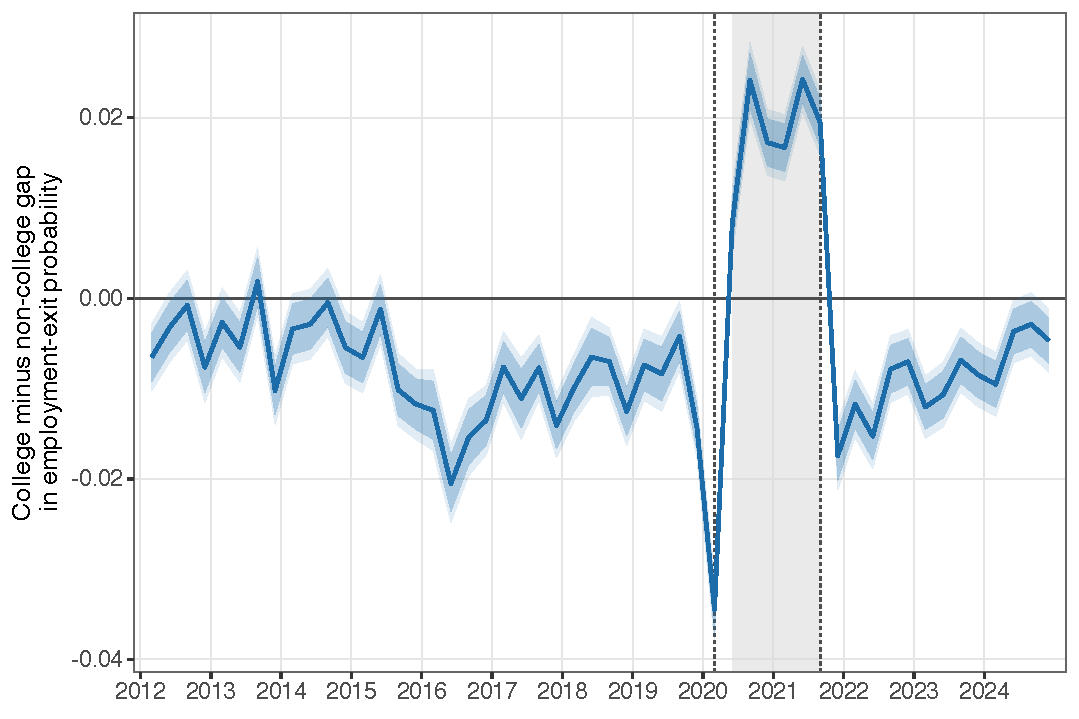
\includegraphics[width=0.86\linewidth]{fig_gap.pdf}
  \caption{College minus non-college difference in the adjusted probability of
  employment exit, \QfirstLab--\QlastLab. Survey-weighted average predictive
  margins from equation~\eqref{eq:es}. The dark band is the pointwise 95\%
  interval; the light band is the sup-$t$ simultaneous band over all
  \Nquarters{} quarterly contrasts (critical value \SuptCrit). Both quantify
  sampling uncertainty conditional on the realised quarter; inference over
  aggregate time shocks is reported only for period averages.}
  \label{fig:gap}
\end{figure}

\begin{table}[H]
\centering
\caption{Adjusted employment-exit probabilities and the college gap, by destination and period}
\label{tab:main_margins}
\begin{threeparttable}
\footnotesize
\renewcommand{\arraystretch}{0.96}
\setlength{\tabcolsep}{4pt}
\begin{tabular}{lccccrr}
\toprule
& \multicolumn{2}{c}{Adjusted level} & \multicolumn{3}{c}{College $-$ no college} & \\
\cmidrule(lr){2-3}\cmidrule(lr){4-6}
& No college & College & Difference & 95\% CI & \multicolumn{2}{c}{\% change vs.\ pre-pandemic} \\
\cmidrule(lr){6-7}
Period & (1) & (2) & (3) & (4) & No college & College \\
\midrule
\multicolumn{7}{l}{\textit{Panel A. Employment exit}} \\
\quad Pre-pandemic & 0.099 & 0.092 & -0.008$^{***}$ & [-0.010, -0.005] & -- & -- \\
 & (0.0002) & (0.0011) & (0.0013) & & & \\
\quad Onset & 0.135 & 0.101 & -0.034$^{***}$ & [-0.037, -0.032] & 36.1 & 10.3 \\
 & (0.0003) & (0.0010) & (0.0013) & & & \\
\quad Mid-pandemic & 0.056 & 0.075 & 0.019$^{***}$ & [0.016, 0.021] & -43.5 & -18.3 \\
 & (0.0003) & (0.0010) & (0.0013) & & & \\
\quad Post-pandemic & 0.097 & 0.088 & -0.009$^{***}$ & [-0.012, -0.007] & -2.5 & -4.4 \\
 & (0.0003) & (0.0010) & (0.0013) & & & \\
\addlinespace
\multicolumn{7}{l}{\textit{Panel B. Exit into unemployment}} \\
\quad Pre-pandemic & 0.031 & 0.029 & -0.002$^{***}$ & [-0.003, -0.001] & -- & -- \\
 & (0.0001) & (0.0005) & (0.0007) & & & \\
\quad Onset & 0.040 & 0.029 & -0.011$^{***}$ & [-0.012, -0.010] & 28.2 & -0.3 \\
 & (0.0002) & (0.0005) & (0.0007) & & & \\
\quad Mid-pandemic & 0.023 & 0.024 & 0.002$^{**}$ & [0.000, 0.003] & -28.0 & -17.6 \\
 & (0.0002) & (0.0005) & (0.0006) & & & \\
\quad Post-pandemic & 0.026 & 0.026 & 0.000 & [-0.001, 0.002] & -17.0 & -9.8 \\
 & (0.0001) & (0.0005) & (0.0006) & & & \\
\addlinespace
\multicolumn{7}{l}{\textit{Panel C. Exit into non-participation}} \\
\quad Pre-pandemic & 0.068 & 0.062 & -0.006$^{***}$ & [-0.008, -0.004] & -- & -- \\
 & (0.0002) & (0.0008) & (0.0010) & & & \\
\quad Onset & 0.095 & 0.072 & -0.023$^{***}$ & [-0.026, -0.021] & 39.8 & 15.3 \\
 & (0.0002) & (0.0008) & (0.0011) & & & \\
\quad Mid-pandemic & 0.034 & 0.051 & 0.017$^{***}$ & [0.015, 0.019] & -50.6 & -18.6 \\
 & (0.0003) & (0.0008) & (0.0010) & & & \\
\quad Post-pandemic & 0.071 & 0.061 & -0.010$^{***}$ & [-0.012, -0.008] & 4.2 & -1.8 \\
 & (0.0002) & (0.0007) & (0.0010) & & & \\
\bottomrule
\end{tabular}
\begin{tablenotes}[flushleft]\scriptsize
\item Notes: Entries in columns (1)--(3) are survey-weighted average predictive margins from the event-study specification of equation~(\ref{eq:es}), which includes year-quarter, state, urban, gender, race, tenure, occupation and sector fixed effects and controls for age, age squared, usual weekly hours, log labour income, formality, temporary status and social security contribution. Margins are computed by holding the covariate distribution fixed and setting the college indicator to zero and to one in turn; they are not regression intercepts. Panel A is any exit from employment; Panels B and C split it by destination, so B and C sum to A by construction. Standard errors in parentheses are two-way clustered by primary sampling unit and year-quarter. Stars on the difference in column (3) denote $^{*}p<0.10$, $^{**}p<0.05$, $^{***}p<0.01$; the adjusted levels are probabilities and carry none. The last two columns report the percentage change in each group's adjusted level relative to its own pre-pandemic average.
\end{tablenotes}
\end{threeparttable}
\end{table}


The series falls into three phases. Through 2012--2019 the gradient is stable
and runs the expected way: the adjusted gap averages \PreGap{} (s.e.\
\PreGapSE), so graduates are about \PreGapAbsPP{} percentage points less likely
to leave employment than otherwise comparable non-graduates. At the onset, in
2020Q1, the gradient widens sharply to \GapOnsetQ: the first wave of exits fell
disproportionately on workers without a degree, whose adjusted exit level rose
\OnsetRelNoCol\% above its pre-pandemic average, against a rise of
\OnsetRelCol\% for graduates. This contrast, however, is identified from a
single quarter. Its asymptotic standard error is small under every clustering
scheme we try, including clustering on year-quarter alone, but that is exactly
the configuration in which the cluster-robust variance is known to be badly
downward biased: the deviation is picked up in one cluster out of \Nquarters{}
\citep{Cameron2008, Roodman2019}. Imposing the null and resampling signs across
quarters, the wild cluster bootstrap fails to reject ($p = \WcbOnset$). A
movement of this size in the education gap in a single quarter is not unusual
once quarterly shocks to the gap are taken seriously. We report the onset
estimate as a description of what happened in 2020Q1 and build nothing on it.

From 2020Q2 the gradient closes and, on the full surveyed population,
overshoots. Over the six quarters to 2021Q3 the adjusted gap averages \MidGap{}
(s.e.\ \MidGapSE, 95\% CI [\MidGapLo, \MidGapHi]), peaking at \GapMaxRev{} in
\GapMaxRevQ. The estimated gap is positive in \NRevQuarters{} of the
\Nquarters{} quarters: the six inside the window, plus an isolated \RevFirst.
The wild cluster bootstrap over year-quarters rejects a zero six-quarter average
comfortably ($p$~\WcbMid).

We are deliberate about what the quarterly path can carry. Each
$\widehat\Delta_q$ is supported by a single year-quarter, so its interval
measures sampling uncertainty conditional on the shocks that quarter realised;
it cannot absorb an education-specific aggregate shock arriving in that same
quarter. The sup-$t$ band corrects the multiplicity of reading \Nquarters{}
contrasts at once, and on that basis it excludes zero in \NRevSimQuarters{}
quarters, all of them inside the window. But a multiplicity correction
conditional on $\widehat V$ does not create temporal replication, which is the
same objection we raise against the onset estimate. Our confirmatory inference
therefore concerns the six-quarter average. Treating the \Nquarters{} quarterly
gaps as the observations and regressing them on a window indicator gives $\tau =
\PlaceboTau{}$ (Newey--West with four lags). The window itself was read off the
estimated series rather than fixed in advance, so we report two things a reader
would otherwise have to take on trust. Moving its end point to 2021Q2 or 2021Q4
leaves the contrast essentially unchanged; and of the \PlaceboNPre{} contiguous
six-quarter windows that lie entirely before 2020Q1, \PlaceboNGE{} reach a
$\tau$ as large, giving a placebo $p$ of \PlaceboPPlacebo. A six-quarter run of
this size is not something this series produces on its own.

Mechanically the movement comes from both sides: the adjusted exit level of
non-graduates falls \MidRelNoColAbs\% below its pre-pandemic average while that
of graduates falls only \MidRelColAbs\%. Exit rates fall for everyone in the
mid-pandemic --- hirings and separations both collapse --- and it is the
gradient that closes. From 2021Q4 the pre-pandemic configuration returns, and by
the end of the sample the adjusted gap is \PostGap.

Table~\ref{tab:spec_ladder} shows how the two pandemic contrasts move as
controls and fixed effects are added, and reports the wild cluster bootstrap
$p$-values for the preferred specification. The ladder is informative in two
ways. Substantively, the pattern appears only in columns (5) and (6): with
quarter, state and demographic controls alone the mid-pandemic gap is still
negative, and it turns positive once time-varying job characteristics and
occupation and sector fixed effects are added. This is the same message the
decomposition delivers in Section~\ref{sec:decomposition}. Statistically, the
mid-pandemic contrast is unambiguous under the year-quarter bootstrap while the
onset contrast is not, for the reason just given: one treated quarter cannot be
separated from a quarterly shock.

\begin{table}[H]
\centering
\caption{The college gap in employment exits across specifications}
\label{tab:spec_ladder}
\begin{threeparttable}
\small
\setlength{\tabcolsep}{4pt}
\begin{tabular}{lcccccc}
\toprule
& (1) & (2) & (3) & (4) & (5) & (6) \\
\midrule
College, other quarters ($\delta$) & -0.069$^{***}$ & -0.069$^{***}$ & -0.060$^{***}$ & -0.053$^{***}$ & -0.023$^{***}$ & -0.010$^{***}$ \\
 & (0.001) & (0.001) & (0.001) & (0.001) & (0.001) & (0.001) \\
\addlinespace
College $\times$ onset ($\omega_1$) & -0.021$^{***}$ & -0.021$^{***}$ & -0.023$^{***}$ & -0.025$^{***}$ & -0.025$^{***}$ & -0.026 \\
 & (0.001) & (0.001) & (0.001) & (0.001) & (0.001) & (0.001) \\
\quad Wild cluster bootstrap $p$ & -- & -- & -- & -- & -- & 0.177 \\
\addlinespace
College $\times$ mid-pandemic ($\omega_2$) & 0.029$^{***}$ & 0.029$^{***}$ & 0.029$^{***}$ & 0.027$^{***}$ & 0.027$^{***}$ & 0.027$^{***}$ \\
 & (0.002) & (0.002) & (0.002) & (0.002) & (0.002) & (0.002) \\
\quad Wild cluster bootstrap $p$ & -- & -- & -- & -- & -- & $<$0.0001 \\
\midrule
\multicolumn{7}{l}{\textit{Implied college gap}} \\
\quad Onset ($\delta+\omega_1$) & -0.090$^{***}$ & -0.090$^{***}$ & -0.083$^{***}$ & -0.077$^{***}$ & -0.048$^{***}$ & -0.035$^{***}$ \\
 & (0.000) & (0.000) & (0.000) & (0.000) & (0.001) & (0.001) \\
\addlinespace
\quad Mid-pandemic ($\delta+\omega_2$) & -0.040$^{***}$ & -0.040$^{***}$ & -0.030$^{***}$ & -0.026$^{***}$ & 0.005$^{**}$ & 0.018$^{***}$ \\
 & (0.002) & (0.002) & (0.002) & (0.002) & (0.002) & (0.002) \\
\midrule
Year-quarter FE & -- & Yes & Yes & Yes & Yes & Yes \\
State and urban FE & -- & -- & Yes & Yes & Yes & Yes \\
Gender and race FE & -- & -- & -- & Yes & Yes & Yes \\
Tenure FE & -- & -- & -- & -- & Yes & Yes \\
Occupation and sector FE & -- & -- & -- & -- & -- & Yes \\
Time-varying job controls & -- & -- & -- & -- & Yes & Yes \\
\addlinespace
Observations & 8,002,128 & 8,002,128 & 8,002,128 & 8,002,128 & 8,002,128 & 8,002,128 \\
$R^2$ & 0.010 & 0.011 & 0.020 & 0.045 & 0.091 & 0.093 \\
\bottomrule
\end{tabular}
\begin{tablenotes}[flushleft]\footnotesize
\item Notes: Survey-weighted linear probability models. The dependent variable is an indicator for exiting employment between $t$ and $t+1$. $\delta$ is the college gap outside the two pandemic windows; $\omega_1$ and $\omega_2$ shift it at the onset and during the mid-pandemic window. Standard errors in parentheses are two-way clustered by primary sampling unit and year-quarter. For the two pandemic deviations we also report, for the preferred specification in column (6), wild cluster bootstrap $p$-values clustered by year-quarter (52 clusters), using Rademacher weights with the null imposed and 9,999 replications; they test $\omega_1$ and $\omega_2$, the shifts in the gap, which is where the number of quarterly shocks rather than the number of records determines uncertainty. Stars denote $^{*}p<0.10$, $^{**}p<0.05$, $^{***}p<0.01$; they are based on the wild cluster bootstrap $p$-value wherever one is reported, and on the asymptotic two-way clustered standard error otherwise. The onset deviation $\omega_1$ therefore carries no stars in column (6): identified from a single year-quarter, it cannot be told apart from an ordinary quarterly shock. The implied gaps keep their asymptotic stars because they are dominated by $\delta$, which is identified across all 52 quarters. Periods are pre-pandemic 2012Q1--2019Q4, onset 2020Q1, mid-pandemic 2020Q2--2021Q3 and post-pandemic 2021Q4--2024Q4.
\end{tablenotes}
\end{threeparttable}
\end{table}


\subsection{Where it happens}\label{sec:where}

Figure~\ref{fig:formal} re-estimates the model separately on formal and on
informal employment. Exit risk is far higher in informal employment throughout,
and the closing of the gradient is an informal-sector phenomenon. Among informal
workers the adjusted gap moves from \InformalPreGap{} before the pandemic to
\InformalMidGap{} (s.e.\ \InformalMidGapSE) in 2020Q2--2021Q3; among formal
workers it moves from \FormalPreGap{} to \FormalMidGap.

\begin{figure}[htbp]
  \centering
  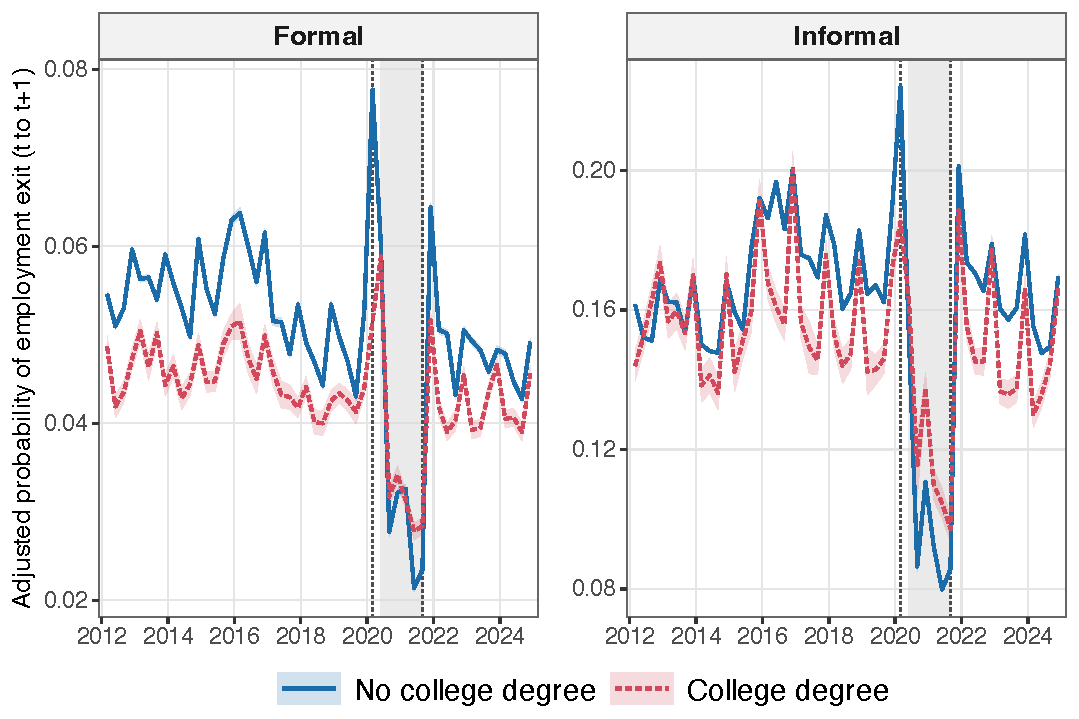
\includegraphics[width=0.86\linewidth]{fig_formal_informal.pdf}
  \caption{Adjusted probability of employment exit by education, formal and
  informal employment estimated separately. Survey-weighted average predictive
  margins from equation~\eqref{eq:es} with 95\% pointwise bands. Note the
  different vertical scales.}
  \label{fig:formal}
\end{figure}

Splitting each side into detailed labour-market positions narrows the locus
further. The movement is driven by informal private employees --- workers in a
dependent employment relationship without a signed work card --- whose adjusted
gap moves from \InfPrivPreGap{} to \InfPrivMidGap. It is absent among the
informal self-employed (\InfSelfMidGap), among formal private employees
(\FormPrivMidGap) and among formal public servants (\FormPubMidGap); only the
formal self-employed show a smaller echo of it (\FormSelfMidGap).
Table~\ref{tab:heterogeneity} reports every segment, together with the
demographic splits discussed below. That the
movement is concentrated among informal employees rather than the informal
self-employed is consistent with a separation channel operating inside dependent
employment relationships, which is where an employer decision can end a job. The
data do not license more than that: our outcome records a transition out of
employment and does not distinguish an employer-initiated dismissal from a
voluntary exit, from discouragement, or from a labour-supply response to the
transfer.

The pattern is not the product of a single demographic group. The pre-pandemic
gradient is not uniform --- it is markedly steeper for women (\WomenPreGap) than
for men (\MenPreGap), and steeper for non-white workers (\NonWhitePreGap) than
for white workers (\WhitePreGap) --- but the mid-pandemic movement appears in
every group, at \MenMidGap{} for men and \WomenMidGap{} for women, and
\WhiteMidGap{} for white and \NonWhiteMidGap{} for non-white workers. Its
magnitude tracks informality: it is largest among women and among non-white
workers, the two groups whose employment is most concentrated in the informal
segment.

\begin{table}[H]
\centering
\caption{Adjusted college gap in employment exits, by labour market segment}
\label{tab:heterogeneity}
\begin{threeparttable}
\small
\setlength{\tabcolsep}{4pt}
\begin{tabular}{lccccr}
\toprule
Segment & Pre-pandemic & Onset & Mid-pandemic & Post-pandemic & Obs. \\
\midrule
\addlinespace\multicolumn{6}{l}{\textit{Formality}} \\
\quad Formal & -0.009$^{***}$ & -0.026$^{***}$ & 0.002$^{***}$ & -0.006$^{***}$ & 4,363,453 \\
 & (0.001) & (0.001) & (0.001) & (0.001) & \\
\quad Informal & -0.014$^{***}$ & -0.040$^{***}$ & 0.019$^{***}$ & -0.019$^{***}$ & 3,638,675 \\
 & (0.002) & (0.003) & (0.002) & (0.002) & \\
\addlinespace\multicolumn{6}{l}{\textit{Gender}} \\
\quad Men & -0.004$^{***}$ & -0.029$^{***}$ & 0.015$^{***}$ & -0.005$^{***}$ & 4,656,560 \\
 & (0.001) & (0.001) & (0.001) & (0.001) & \\
\quad Women & -0.013$^{***}$ & -0.043$^{***}$ & 0.025$^{***}$ & -0.016$^{***}$ & 3,345,568 \\
 & (0.002) & (0.002) & (0.002) & (0.002) & \\
\addlinespace\multicolumn{6}{l}{\textit{Position}} \\
\quad Formal private employee & -0.009$^{***}$ & -0.027$^{***}$ & 0.000 & -0.006$^{***}$ & 2,679,329 \\
 & (0.001) & (0.001) & (0.001) & (0.001) & \\
\quad Formal public sector & -0.004$^{***}$ & -0.007$^{***}$ & -0.003$^{***}$ & -0.007$^{***}$ & 818,008 \\
 & (0.001) & (0.001) & (0.001) & (0.001) & \\
\quad Formal self-employed & -0.005$^{***}$ & -0.003 & 0.008$^{***}$ & -0.011$^{***}$ & 624,666 \\
 & (0.002) & (0.003) & (0.002) & (0.001) & \\
\quad Informal private employee & -0.015$^{***}$ & -0.045$^{***}$ & 0.029$^{***}$ & -0.015$^{***}$ & 1,674,121 \\
 & (0.002) & (0.004) & (0.003) & (0.002) & \\
\quad Informal self-employed & -0.014$^{***}$ & -0.027$^{***}$ & -0.001 & -0.022$^{***}$ & 1,621,692 \\
 & (0.002) & (0.004) & (0.003) & (0.002) & \\
\addlinespace\multicolumn{6}{l}{\textit{Race}} \\
\quad Non-White & -0.013$^{***}$ & -0.032$^{***}$ & 0.022$^{***}$ & -0.013$^{***}$ & 4,582,254 \\
 & (0.001) & (0.002) & (0.002) & (0.001) & \\
\quad White & -0.009$^{***}$ & -0.034$^{***}$ & 0.010$^{***}$ & -0.009$^{***}$ & 3,419,874 \\
 & (0.001) & (0.001) & (0.001) & (0.001) & \\
\bottomrule
\end{tabular}
\begin{tablenotes}[flushleft]\footnotesize
\item Notes: Each cell is the survey-weighted average predictive difference in the probability of exiting employment between workers with and without a college degree, estimated on the indicated subsample with the full specification of equation~(\ref{eq:es}). Fixed effects and controls that are collinear within a segment are dropped. Standard errors in parentheses are two-way clustered by primary sampling unit and year-quarter. Stars denote $^{*}p<0.10$, $^{**}p<0.05$, $^{***}p<0.01$. Periods are pre-pandemic 2012Q1--2019Q4, onset 2020Q1, mid-pandemic 2020Q2--2021Q3 and post-pandemic 2021Q4--2024Q4.
\end{tablenotes}
\end{threeparttable}
\end{table}


\subsection{Composition or within-cell risk?}\label{sec:decomposition}

The decomposition in equation~\eqref{eq:decomp} separates the two explanations,
and neither component dominates. Composition accounts for \DecPreCompShare\% of
the unconditional pre-pandemic gap (\DecPreComp{} out of \DecPreTotal) and
within-cell risk for the remaining \DecPreWithinShare\% (\DecPreWithin), and
those shares are essentially unchanged in every other period and under a finer
partition that also splits cells by labour-market position. Graduates are safer
partly because they hold formal jobs in more protected occupations and sectors,
and partly because they are safer inside those jobs.

What happens during the pandemic is more informative: the two components
compress together during 2020Q2--2021Q3, composition by \DecCompShrink\% and
within-cell risk by \DecWithinShrink\%. The unconditional gap therefore halves,
from \DecPreTotal{} to \DecMidTotal, without changing sign, and the split
between the two components is the same before, during and after. Whether either
group moved towards cells that carried more risk to begin with, the
decomposition cannot say, because the composition component mixes both groups'
shares with rates that are themselves moving. An index that holds the
pre-pandemic cell rates fixed and lets only allocation move, $R_g = \sum_k
(s_{gk,\text{mid}} - s_{gk,\text{pre}})\bar m_{k,\text{pre}}$, answers it
directly. Both indices are positive and the graduates' is the larger, $R_C =
\RealocCollege$ against $R_N = \RealocNonCollege$: graduates did move towards
cells that had carried more risk. The magnitude settles the reading, however:
$R_C$ is smaller than the \DecPreTotal{} gap it would have to explain by a
factor of \RealocShare, so reallocation is present but far too small to be the
mechanism. Reporting the decomposition under the opposite and the symmetric
reference convention, and on common support only, moves the mid-pandemic
composition component only between \DecVarCompLo{} and \DecVarCompHi, so the
split does not rest on the reference chosen.

This pins down what Figure~\ref{fig:gap} shows. It is not visible at the level
of formality, sector and occupation, where the education advantage merely
shrinks by about half. It emerges only once the richer conditioning set of
equation~\eqref{eq:es} is applied, that is, once two workers are matched not
only on cell but also on hours, labour income, tenure, contract type, social
security status and location. Inside a given formality-sector-occupation cell,
graduates still hold the better-paid, longer-tenured, contractually protected
jobs. Strip that residual advantage away as well and, for six quarters, their
edge in staying employed disappears.

%==============================================================================
\section{Selection, common support and robustness}\label{sec:robustness}
%==============================================================================

\paragraph{Panel retention.}
The outcome exists only for workers the matching algorithm finds again, so
differential retention is a first-order concern. Here it is observed directly:
the build keeps every worker employed in quarter $t$, whether or not the
algorithm finds them again, so the indicator we model is the very object at
issue rather than a stand-in for it. One restriction applies --- a worker
observed in the fifth interview has no $t+1$ inside the panel, which is a
scheduled exit rather than attrition, and the survey's own interview counter
identifies those rows exactly. Graduates are consistently easier to re-find, and
the pandemic widened the gap: the college / non-college difference in the match
rate is \RetDiffPre{} before the pandemic, jumps to \RetDiffOnset{} in 2020Q1
when fieldwork switched to telephone interviewing, and is still \RetDiffMid{}
through 2020Q2--2021Q3. We do not dismiss the concern by appealing to its
direction, because the direction is unfavourable: the workers who drop out of
view carry the higher exit risk and are disproportionately non-graduates, so the
mid-pandemic gap we estimate is, if anything, too positive. It has to be bounded
rather than signed away, and we bound it twice. A separate logit per quarter, on
education, demographics, job characteristics and state, occupation and sector
fixed effects, gives each worker a predicted probability of being matched
forward; multiplying the survey weight by the inverse of that probability,
trimmed at 0.05, and re-estimating equation~\eqref{eq:es} leaves the
mid-pandemic gap essentially unchanged, at \IpwMidGapFour{} against
\BaseMidGapFour{} without the re-weighting on the same sample. And imputing an
outcome for every unmatched origin, then shifting it for graduates on the
log-odds scale, reveals no tipping point: pushing the shift to \TippingDeltaMin,
which drives the imputed exit probability of unmatched graduates to essentially
zero from the \TippingRateMAR{} their observed characteristics imply, moves the
mid-pandemic gap only to \TippingFloor.

\paragraph{Common support.}
One check goes to the estimand rather than to its variance, and it is the one
that qualifies the result most. Because the pattern appears only after
conditioning on job characteristics, how far the two education groups overlap on
those characteristics matters: a linear model extrapolates happily into regions
where one group is hardly observed. Table~\ref{tab:overlap} estimates the
propensity to hold a degree quarter by quarter, on the covariates and fixed
effects of equation~\eqref{eq:es}, and reports two departures from the
survey-weighted estimate, which answer different questions. Trimming to
propensities inside $[0.10, 0.90]$ keeps the estimand and drops only the workers
with no counterpart, at the cost of retaining \TrimShare\% of the sample.
Overlap weighting keeps every worker but re-centres the estimand on the region
where a degree is a coin flip.

\begin{table}[H]
\centering
\caption{Common support and overlap-weighted estimates}
\label{tab:overlap}
\begin{threeparttable}
\begin{tabular}{lccccc}
\toprule
& \multicolumn{2}{c}{Support} & \multicolumn{3}{c}{Adjusted gap} \\
\cmidrule(lr){2-3}\cmidrule(lr){4-6}
Period & Off support (\%) & ESS ratio (\%) & Survey w. & Trimmed & Overlap w. \\
\midrule
\multicolumn{6}{l}{\textit{All employment}} \\
\quad Pre-pandemic & 36.0 & 24.6 & -0.0077 & -0.0082 & -0.0094 \\
\quad Onset & 17.6 & 29.6 & -0.0345 & -0.0263 & -0.0175 \\
\quad Mid-pandemic & 17.0 & 31.8 & 0.0184 & -0.0027 & -0.0050 \\
\quad Post-pandemic & 17.7 & 33.5 & -0.0089 & -0.0084 & -0.0095 \\
\addlinespace
\multicolumn{6}{l}{\textit{Informal employment}} \\
\quad Pre-pandemic & 54.9 & 14.0 & -0.0117 & -0.0159 & -0.0127 \\
\quad Onset & 32.4 & 14.9 & -0.0386 & -0.0477 & -0.0145 \\
\quad Mid-pandemic & 31.6 & 21.8 & 0.0196 & 0.0008 & -0.0075 \\
\quad Post-pandemic & 30.7 & 22.5 & -0.0159 & -0.0183 & -0.0148 \\
\bottomrule
\end{tabular}
\begin{tablenotes}[flushleft]\footnotesize
\item Notes: The propensity to hold a college degree is estimated separately in each quarter, on the covariates and fixed effects of equation~\eqref{eq:es}, so that every coefficient may move over time. Overlap weights are $w_i(1-e_i)$ for graduates and $w_i e_i$ for non-graduates, where $e_i$ is that propensity; they weight each cell by how evenly the two education groups populate it and vanish where a cell is effectively single-group. Off support is the survey-weighted share of observations with $e_i$ outside $[0.02, 0.98]$. The ESS ratio is the Kish effective sample size under overlap weights as a share of the same measure under survey weights. The trimmed column keeps the survey-weighted estimand and drops only observations whose propensity falls outside $[0.10, 0.90]$, separating the removal of unsupported comparisons from the re-centring of the estimand that the overlap column performs. Both columns of gaps are estimated on the observations that receive a propensity score, so the two differ only in the weighting. The lower block repeats the exercise inside informal employment, where the two education groups overlap on characteristics that they do not overlap on across the labour market as a whole.
\end{tablenotes}
\end{threeparttable}
\end{table}


Overlap is limited: in 2020Q2--2021Q3, \OverlapMidGapOff\% of the sample carries
a propensity outside $[0.02, 0.98]$ and overlap weighting retains only
\OverlapEssRatio\% of the effective sample size. The two corrections agree, and
they place the positive sign outside the region of common support. Trimmed, the
mid-pandemic gap is \TrimMidGap{} rather than \BaseOverlapMidGap; under overlap
weights it is \OverlapMidGap. Inside informal employment the same holds and
overlap is worse, not better, with \OverlapInfOffSupport\% of the segment off
support: the trimmed gap is \TrimInfMidGap{} (s.e.\ \TrimInfMidSE) against
\BaseOverlapInfMidGap{} on the full segment. Graduates are uncommon in informal
wage employment, so requiring the two groups to be comparable leaves few
comparisons to make.

We read this as a limit on the sign, not on the finding. What survives every
weighting is that the gradient closes: from \TrimPreGap{} to \TrimMidGap{} on
common support overall, and from \TrimInfPreGap{} --- precisely estimated and
clearly negative --- to a mid-pandemic value indistinguishable from zero inside
informal employment. That the point estimate on the full surveyed population
goes further and turns positive is a property of a comparison drawn partly
outside common support, and we do not build on it.

\paragraph{Remaining checks.}
The remaining results are reported in the full version and summarised here.
Restricting to prime-age workers aged 25--54 removes retirement and schooling
transitions from the outcome and leaves the pattern intact; dropping the survey
weights and moving the base quarter to 2019Q1 do the same. Replacing the outcome
by an indicator for being informally employed in $t+1$ shows the complementary
margin of adjustment: there the education gradient runs the usual way throughout
and widens during the window, from \PreGapInf{} to \MidGapInf, so graduates who
kept working became relatively less exposed to informal employment just as their
advantage in staying employed at all disappeared. The two pandemic contrasts are
also robust to the choice of variance estimator --- clustering by PSU, by
household, by individual, by individual and year-quarter, and by year-quarter
alone, the most conservative option available given \Nquarters{} clusters.

%==============================================================================
\section{Discussion and conclusion}\label{sec:conclusion}
%==============================================================================

Using \Nobs{} matched person-quarters from \textit{PNAD Cont\'inua} over
\QfirstLab--\QlastLab, we document that the covariate-adjusted college /
non-college difference in employment exits vanished for six quarters between
2020Q2 and 2021Q3 and then returned to its pre-pandemic configuration, even
though the unconditional education gradient stayed negative throughout. The
single-quarter widening at the onset, though large in point estimate, does not
survive inference clustered on time and we do not build on it. The pattern is
present in adjusted margins computed with survey weights and two-way clustering,
runs entirely through exits out of the labour force rather than into measured
unemployment, is concentrated in informal wage employment, and survives
weighting by the inverse probability of being matched into the following
quarter. Restricted to workers with common support the gradient closes to zero
rather than crossing it, so the disappearance is the robust finding and the sign
of the crossing is not.

Schooling protects Brazilian workers from employment exits through two channels
of comparable size: placement into formal jobs in more protected occupations and
sectors, and a residual advantage inside those cells. Neither dominates, their
relative weights are stable over time, and during 2020Q2--2021Q3 both compressed
by roughly the same proportion --- \DecCompShrink\% and \DecWithinShrink\% ---
halving the unconditional gap without reversing it. What happened is therefore a
statement about workers matched on job characteristics, not about reallocation
across sectors.

The timing is consistent with, but does not identify, a role for the emergency
programmes. \textit{Aux\'ilio Emergencial} started in April 2020 and ended in
October 2021, bracketing the window almost exactly, and it reached the informal,
lower-education workers whose adjusted exit risk fell most; the
employment-preservation programme worked on the formal side, where we find much
smaller movements. But the design has no eligibility discontinuity and no
pre-determined exposure measure, so we cannot separate the programmes from
everything else that moved at the same time: sectoral shutdowns, differential
remote-work feasibility \citep{Dingel2020}, changed labour supply of graduates
with children \citep{Alon2020}, or the composition of who kept searching. The
United States experience with pandemic unemployment benefits illustrates how
sharply such programmes can alter measured transitions even when they are not
designed to \citep{Ganong2020, Marinescu2021}. Claims that ``policy design
matters'' go beyond what this evidence supports; what it supports is that the
education gradient in job security is not a structural constant, and that it
moved in the segment of the labour market where the segmented policy response
was concentrated.

Two limitations remain. The design is descriptive: we observe that the gradient
closed in informal wage employment over the window in which the emergency
transfer operated, but we do not observe anyone who was ineligible for it, and
nothing here rules out a coincident shock with the same timing and the same
incidence. The second is about the comparison itself. The adjusted gap is a
conditional contrast, and the two education groups overlap only partially on the
characteristics we condition on: \TrimShare\% of the sample survives a trim to
propensities inside $[0.10, 0.90]$. Restricted to those workers the gradient
still closes during the window, but it stops at zero instead of crossing it.
Readers who want a contrast between graduates and non-graduates alike in every
measured respect should read the trimmed column of Table~\ref{tab:overlap}, and
it says the advantage went to zero.

The transferable lesson is about the architecture of emergency support rather
than about Brazil. When protection is delivered through two channels that are
segmented along the formal--informal margin, and when schooling predicts which
channel a worker falls into, the aggregate relationship between education and
job security can temporarily detach. Any country with a large informal sector
and a bifurcated safety net has the same structure.

%==============================================================================
\bibliographystyle{elsarticle-harv}
\bibliography{refs}

\end{document}
